\begin{python}
    self.dashboard <= w.label('Select', typo='headline4', style=flex)
    self.dashboard <= w.select(
        'Select',
        [[f'sel-{i}', f'sel-{i}'] for i in range(4)],
        on_change=self.on_select,
        id='my_select',
    )
    self.dashboard <= w.label(
        f'', id='for_select', typo=f'body1', style=flex
    )


def on_select(self, value):
    # value = w.get_value('my_select')
    document.select_one('#for_select').html = f'Select Changed: {value}'
\end{python}


\begin{figure}[H]
\begin{centering}
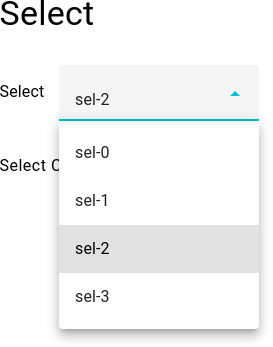
\includegraphics[scale=0.5]{Cap4/Figures/widgets/select.png}
\par\end{centering}
\caption[Brython Radiant: Select]{Brython Radiant: Select.}
\label{fig:radiant_select}
\end{figure}